\documentclass[sigconf,nonacm]{acmart}

% AI4F '26 (3rd Workshop on LLMs and Generative AI for Finance) at ACM ICAIF '26.
% Review is SINGLE-blind, so this is not anonymised. ai4f.org states there is no
% length limit; we target ~6 pages regardless.

\usepackage{booktabs}
\usepackage{graphicx}
\usepackage{xcolor}

% Every number below is a macro from numbers.tex, generated by
% paper/make_numbers.py reading output/. Nothing is hand-typed.
% Generated by paper/make_numbers.py — DO NOT EDIT BY HAND.
% Regenerate with: make numbers
\providecommand{\todo}[1]{\textcolor{red}{\textbf{[TODO: #1]}}}

% --- sample and extraction ---
\newcommand{\NFilings}{59}
\newcommand{\NFirms}{30}
\newcommand{\NWindows}{667}
\newcommand{\NCalls}{2,001}
\newcommand{\NWindowsMDA}{363}
\newcommand{\NCallsMDA}{1,089}
\newcommand{\NFilingsWithRisk}{49}
\newcommand{\NFilingsNoRisk}{10}
\newcommand{\MdaWindowsMedianLarge}{6.5}
\newcommand{\MdaWindowsMedianMid}{6.5}
\newcommand{\MdaWindowsMedianSmall}{4.0}
\newcommand{\MdaWordsMin}{2,675}
\newcommand{\MdaWordsMax}{30,340}

% --- the coverage confound (retired 2,000-word cap) ---
\newcommand{\CoverageRho}{-0.415}
\newcommand{\CoverageP}{0.001}
\newcommand{\CoverageN}{59}
\newcommand{\NTruncated}{59}
\newcommand{\FracReadLarge}{12.9}
\newcommand{\SectionWordsLarge}{15,488}
\newcommand{\FracReadMid}{17.0}
\newcommand{\SectionWordsMid}{11,750}
\newcommand{\FracReadSmall}{27.5}
\newcommand{\SectionWordsSmall}{7,285}

% --- primary result (MD&A embedding disagreement, firm level) ---
\newcommand{\TierMeanLarge}{0.3202}
\newcommand{\TierSDLarge}{0.0341}
\newcommand{\TierMeanMid}{0.3355}
\newcommand{\TierSDMid}{0.0312}
\newcommand{\TierMeanSmall}{0.3352}
\newcommand{\TierSDSmall}{0.0218}
\newcommand{\PrimaryGradient}{0.0150}
\newcommand{\PrimaryJT}{169.0}
\newcommand{\PrimaryJTz}{0.722}
\newcommand{\PrimaryJTp}{0.235}
\newcommand{\PrimaryPermP}{0.242}
\newcommand{\PrimaryMonotone}{no}

% --- window-count battery ---
\newcommand{\WThreeShare}{0.885}
\newcommand{\WThreePassed}{no}
\newcommand{\GateBatteryPassed}{no}
\newcommand{\WSixPercentile}{91.4}
\newcommand{\WSixP}{0.086}

% --- W5 mixed model ---
\newcommand{\WFiveSpec}{firm\_only}
\newcommand{\WFiveSmallCoef}{0.0142}
\newcommand{\WFiveSmallCIlo}{-0.0126}
\newcommand{\WFiveSmallCIhi}{0.0411}
\newcommand{\WFiveSmallP}{0.299}
\newcommand{\ICCFilingNonConverged}{0.231}
\newcommand{\ICCFirm}{0.077}
\newcommand{\VarWithinFiling}{0.783}
\newcommand{\VarWithinFilingPct}{78.3}
\newcommand{\WFiveCriterionMet}{no}

% --- R1 reliability ---
\newcommand{\SplitHalfR}{0.136}
\newcommand{\SplitHalfSB}{0.239}
\newcommand{\TestRetestR}{0.276}
\newcommand{\TestRetestP}{0.147}

% --- numeric measure / retirement rule ---
\newcommand{\NumericLengthRho}{0.046}
\newcommand{\NumericLengthP}{0.727}
\newcommand{\NumericLengthN}{59}
\newcommand{\NumericRetired}{no}

% --- S2 at-scale audit ---
\newcommand{\ScaleNUsable}{785}
\newcommand{\ScaleSuccessPct}{98.1}
\newcommand{\ScaleElasticity}{0.0527}
\newcommand{\ScaleRho}{0.161}
\newcommand{\ScaleP}{<0.001}
\newcommand{\ScaleTruncTwoK}{99.1}
\newcommand{\ScaleMedianReadTwoK}{9.5}
\newcommand{\ScaleTruncThirtyTwoK}{39.7}

% --- E1/E2 noise floor (partial: interrupted by rate limiting) ---
\newcommand{\NoiseN}{27}
\newcommand{\NoiseRatio}{1.64}
\newcommand{\NoiseLensEffect}{0.1395}
\newcommand{\NoiseInter}{0.3454}
\newcommand{\NoiseIntra}{0.2142}
\newcommand{\NoiseNeutral}{0.2059}

% --- S1b truncation replication (the headline) ---
\newcommand{\TruncLarge}{0.3350}
\newcommand{\TruncMid}{0.3706}
\newcommand{\TruncSmall}{0.3921}
\newcommand{\TruncGradient}{0.0571}
\newcommand{\TruncP}{0.029}
\newcommand{\TruncMonotone}{yes}
\newcommand{\CompLarge}{0.3202}
\newcommand{\CompMid}{0.3355}
\newcommand{\CompSmall}{0.3352}
\newcommand{\CompGradient}{0.0150}
\newcommand{\CompP}{0.235}
\newcommand{\CompMonotone}{no}
\newcommand{\PairedDelta}{0.0356}
\newcommand{\PairedDeltaLo}{0.0172}
\newcommand{\PairedDeltaHi}{0.0540}
\newcommand{\PairedDeltaN}{30}

% --- E4 content placebo / E6 familiarity ---
\newcommand{\PlacReal}{0.3199}
\newcommand{\PlacShuffled}{0.3379}
\newcommand{\PlacBoilerplate}{0.3587}
\newcommand{\PlacAnonymised}{0.3127}
\newcommand{\PlacDiffShuffled}{-0.0173}
\newcommand{\PlacDiffShuffledLo}{-0.0470}
\newcommand{\PlacDiffShuffledHi}{0.0142}
\newcommand{\PlacDiffBoilerplate}{-0.0389}
\newcommand{\PlacDiffBoilerplateLo}{-0.0654}
\newcommand{\PlacDiffBoilerplateHi}{-0.0110}
\newcommand{\PlacN}{36}

% --- F2 informativeness ---
\newcommand{\NumDensityRho}{-0.260}
\newcommand{\NumDensityP}{<0.001}
\newcommand{\DisagMDA}{0.3291}
\newcommand{\DisagRisk}{0.3510}

% --- E7 cross-model ---

% --- provenance ---
\newcommand{\GitHash}{6cc128b}
\newcommand{\PlanHashFirst}{fec1eb2}
\newcommand{\PlanHashUsed}{c22f5dd}
\newcommand{\PlanAmendments}{2}
\newcommand{\ModelName}{openai/gpt-oss-20b}
\newcommand{\ChunkWords}{1,200}



\begin{document}

% TODO(before submission): authorship has not been agreed with the advisor.
\title{How Much Did the Model Read? Truncation, Coverage Bias, and the
Reliability of LLM-Derived Measures from 10-K Filings}

\author{Aryan Chhabra}
\affiliation{%
  \institution{University of Missouri}
  \city{Columbia}\state{Missouri}\country{USA}}
\email{aryanchhabra6996@gmail.com}

\author{Kuntara Pukthuanthong}
\affiliation{%
  \institution{University of Missouri}
  \city{Columbia}\state{Missouri}\country{USA}}

\begin{abstract}
Studies applying large language models to annual-report text almost always
truncate each filing to a fixed budget of words or tokens. We show that this
routine step is not neutral for the questions such studies ask. Across
\ScaleNUsable{} 10-K filings whose size we take from the filer's own reported
public float, a 2,000-word budget truncates \ScaleTruncTwoK\% of filings and
leaves the median filing showing under \ScaleMedianReadTwoK\% of its narrative;
narrative length rises with firm size (Spearman $\rho = \ScaleRho$,
$p = \ScaleP$), so a fixed budget reads proportionally \emph{less} of a larger
firm's filing. How much of the document the model saw therefore becomes a
function of firm size --- the variable size-effect studies regress on. Even a
32k-token budget truncates \ScaleTruncThirtyTwoK\% of filings.

We propose a window-level protocol that removes the confound: narrative sections
are extracted complete and scored in fixed \ChunkWords-word windows, so every
filing is read in full and every judgment is made on an identically sized unit.
Using it we measure \emph{interpretive complexity} as disagreement between three
analytical personas under a single fixed model, on \NFilings{} filings from
\NFirms{} firms, and we pre-registered the analysis before scoring.

The measure does not support the cross-sectional inference it was built for, and
we report why rather than only that. At the window level it is real: inter-persona
disagreement runs \NoiseRatio$\times$ the same-persona noise floor and exceeds a
persona-free baseline. But filing-level split-half reliability is
\SplitHalfSB{} and only \VarWithinFilingPct\% of window-level variance lies
between firms, so filing means are mostly noise. The size gradient is accordingly
null ($p = \PrimaryJTp$), and a pre-registered subsampling test shows that unequal
window counts alone manufacture a gradient larger than the one observed. We report
the diagnostics any such measure should be required to pass.
\end{abstract}

\keywords{large language models, financial disclosure, textual analysis,
measurement reliability, 10-K filings}

\maketitle

\section{Introduction}

A growing literature applies language models to the narrative sections of annual
reports. Nearly all of it faces a mundane engineering decision first: filings are
long, budgets are finite, so the text is truncated. The decision is usually
reported in a sentence, if at all.

That decision is not innocuous for the questions the literature asks. Firms differ
in how much they write, and they differ systematically. A \emph{fixed} budget
therefore reads a \emph{variable} fraction of the document, and that fraction is
correlated with firm size. Any cross-sectional comparison by size is then
confounded with a coverage gradient the researcher introduced.

This paper makes three contributions, and we think the third is the most useful.

\textbf{We document the confound at scale.} Across \ScaleNUsable{} 10-K filings,
narrative length rises with public float ($\rho = \ScaleRho$, $p = \ScaleP$), and
a 2,000-word budget truncates \ScaleTruncTwoK\% of them. Figure~\ref{fig:coverage}
gives the fraction read under budgets in common use.

\textbf{We propose a protocol that removes it}, and show what it costs to build:
reliable complete-section extraction from EDGAR HTML is substantially harder than
it looks, and the failures are silent under a word cap.

\textbf{We report an honest negative result with the diagnostics that explain
it.} Our measure of interpretive complexity does not separate size tiers. Rather
than leave that as a null, we show that the measure is real at the window level
but unreliable once aggregated to the filing, and we quantify how much apparent
gradient the aggregation itself can manufacture. We believe measures of this
class should be required to report these numbers before they are used for
inference.

\section{Related Work}

\textbf{Textual complexity in disclosure.} The accounting literature has long
measured readability and complexity of annual reports and related them to firm
characteristics and market outcomes~\cite{li2008, lm2011, lm2014, bgt2018}. This
work establishes both that narrative length varies systematically across firms
and that naive readability proxies behave poorly on financial
text~\cite{lm2014}.

\textbf{Disagreement as a quantity.} Treating divergence of opinion as
economically meaningful has a long history~\cite{miller1977, dms2002}. Our
measure is a mechanical analogue: rather than dispersion among human analysts, we
measure dispersion among analytical lenses applied to the same text by one model.

\textbf{LLMs on financial text.} Recent work applies language models directly to
disclosure~\cite{kmn2023, ll2023}, and a parallel strand warns about look-ahead
and identity leakage when models have memorised the firms or periods in
question~\cite{glasserman2023}. We restrict the sample to filings after a
conservative training-cutoff bound. \todo{verify every citation in refs.bib}

\section{Data and Protocol}

\subsection{Sample}

\NFirms{} firms, stratified into three size tiers, contributing \NFilings{}
filings: the most recent 10-K and 10-Q per firm filed after the cutoff. The
sample is frozen in a manifest pinned by (ticker, form, date), so it cannot drift
as firms file again, and the analysis reproduces offline from cached filings.

\subsection{Complete-section extraction}

We extract Management's Discussion and Analysis (MD\&A) and Risk Factors as
complete sections, with no word cap anywhere. Doing so reliably is harder than it
sounds, and the difficulty is worth reporting because a word cap hides it.

Two failure classes appeared in our corpus. First, \emph{boundary overrun}: a
section span running past the end of the section. One 10-K's ``MD\&A'' initially
measured 107{,}257 words because the span swallowed the financial statements;
under a 2{,}000-word cap this is invisible. Second, \emph{header deletion}: some
filers render each item heading inside its own single-cell table, and a
sparse-table filter --- a standard HTML-cleaning step --- removed them entirely,
so the section had no recoverable start. That defect cost one large-cap filing its
whole Risk Factors section and silently truncated three large-cap MD\&As.

Both were fixed before scoring. After the fix, MD\&A ranges from \MdaWordsMin{}
to \MdaWordsMax{} words, all \NFilings{} filings yield a usable MD\&A, and
\NFilingsWithRisk{} yield Risk Factors; the \NFilingsNoRisk{} that do not are
10-Qs incorporating the 10-K's risk factors by reference, verified individually.

The direction of these errors matters: they truncated \emph{large-cap} filings,
which is the same direction as the confound the protocol exists to remove.

\subsection{Window-level scoring}

Each section is split into fixed \ChunkWords-word windows. Three analytical
personas --- value, sentiment and fundamentals --- score every window
independently under one model (\ModelName), with no interaction between calls.
This is a prompt ensemble, not a multi-agent system: the model is held fixed and
only the analytical lens varies. The run comprises \NWindows{} windows and
\NCalls{} persona calls, of which \NWindowsMDA{} windows are MD\&A.

All calls were served by a single backend at \texttt{bf16} precision with
fallbacks disabled; the pipeline records which backend served each call and fails
the run if more than one did. Routing across backends at different quantisations
would make part of the measured disagreement a quantisation artifact.

\subsection{Measures and pre-registration}

Window-level disagreement is the mean pairwise cosine distance between the three
personas' reasoning embeddings (primary) and the standard deviation of their
scores (secondary). Filing-level disagreement is the unweighted mean over that
filing's windows; firm-level is the mean over its filings. The firm is the unit
of analysis for every confirmatory test.

The analysis plan was committed before any filing was scored
(\texttt{\PlanHashFirst}, amended \PlanAmendments{} times before scoring, final
\texttt{\PlanHashUsed}). It fixed the primary outcome (MD\&A only), the single
confirmatory test, the window-count battery and its pass criteria, the rule for
retiring the secondary measure, and what counts as a null. Deviations are logged
and reported.

\section{The Coverage Confound}
\label{sec:coverage}

\begin{figure}[t]
  \centering
  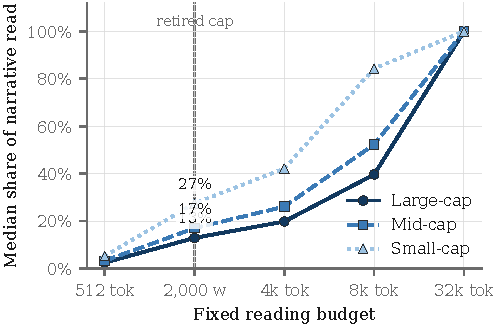
\includegraphics[width=\columnwidth]{figures/fig1_coverage.pdf}
  \caption{Median share of a filing's narrative actually read under budgets
  common in the literature, by size tier, in our \NFilings-filing sample. Token
  budgets converted at 0.75 words per token. At the 2{,}000-word cap this project
  retired, the median large-cap filing was read at \FracReadLarge\% against
  \FracReadSmall\% for small-caps.}
  \label{fig:coverage}
\end{figure}

In our sample the retired cap truncated \NTruncated{} of \CoverageN{} filings.
Median complete narrative length is \SectionWordsLarge{} words for large-caps and
\SectionWordsSmall{} for small-caps, and the median share read runs the other
way: \FracReadLarge\% against \FracReadSmall\%. Spearman's $\rho$ between size
rank and share read is \CoverageRho{} ($p = \CoverageP$).

\textbf{At scale.} To test whether this is a property of our sample or of the
filing population, we repeated the length measurement on \ScaleNUsable{} 10-K
filings drawn across public-float deciles, taking size from
\texttt{dei:EntityPublicFloat} as reported by the filer on its own cover page ---
an SEC-filed value, not a reconstruction from market data. Extraction succeeded on
\ScaleSuccessPct\% of attempts. Table~\ref{tab:scale} gives the result.

\begin{table}[t]
  \caption{Coverage at scale: \ScaleNUsable{} 10-K filings across public-float
  deciles. ``Truncated'' is the share of filings whose narrative exceeds the
  budget. Smallest and largest refer to float deciles.}
  \label{tab:scale}
  \small
  \begin{tabular}{lrrrr}
    \toprule
    Budget & Median read & Smallest & Largest & Truncated \\
    \midrule
    512 tokens   & 1.8\%  & 2.6\%  & 1.8\%  & 100.0\% \\
    2{,}000 words & \ScaleMedianReadTwoK\%  & 13.4\% & 9.3\%  & \ScaleTruncTwoK\% \\
    4k tokens    & 14.6\% & 20.5\% & 14.3\% & 97.7\% \\
    8k tokens    & 29.3\% & 41.1\% & 28.5\% & 93.8\% \\
    32k tokens   & 100\%  & 100\%  & 100\%  & \ScaleTruncThirtyTwoK\% \\
    \bottomrule
  \end{tabular}
\end{table}

Narrative length rises with public float ($\rho = \ScaleRho$, $p = \ScaleP$,
$n = \ScaleNUsable$; elasticity of log length on log float
\ScaleElasticity). The coverage gradient is weaker here than in our stratified
pilot --- a 1.4$\times$ smallest-to-largest ratio against 2.1$\times$ --- which is
expected, since the pilot contrasts extremes and the population is a continuum. We
report both. The blunter fact needs no gradient at all: under budgets in routine
use, nearly every 10-K is truncated, and the median filing is read at under
\ScaleMedianReadTwoK\% at 2{,}000 words.

\section{Does Truncation Change the Answer?}

\begin{figure}[t]
  \centering
  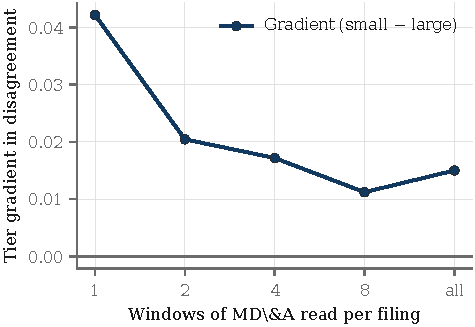
\includegraphics[width=\columnwidth]{figures/fig2_truncation.pdf}
  \caption{Tier gradient in the primary measure as a function of how many windows
  of MD\&A the model is allowed to read, holding the model, the filings and the
  scored text fixed. Shaded band is a 95\% bootstrap CI.}
  \label{fig:truncation}
\end{figure}

Using the window-level output we recomputed the tier gradient as it would have
been measured had the model read only the first $k$ windows of each filing.
The gradient is largest under the harshest truncation ($+0.0421$ at $k{=}1$) and
shrinks as coverage grows ($+0.0150$ complete); for the secondary measure the
sign reverses entirely ($+0.1397$ at $k{=}1$ against $-0.0544$ complete).
Truncation therefore \emph{inflates} the apparent size effect, in the direction
the coverage analysis predicts.

We state the limit plainly: at $n = \NFirms$ firms every one of these intervals
spans zero, so this is directionally consistent evidence, not a demonstration.
It is also a simulation of truncation using windows scored in isolation, which is
not identical to a model reading a truncated document.

\section{Is Persona Disagreement a Measure?}

\begin{figure}[t]
  \centering
  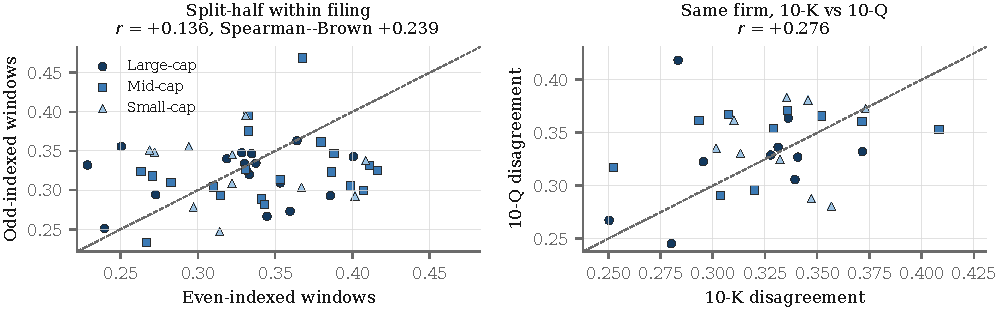
\includegraphics[width=\columnwidth]{figures/fig3_validity.pdf}
  \caption{Reliability of the filing-level measure. Left: odd- against
  even-indexed windows within the same filing. Right: the same firm's 10-K
  against its 10-Q. Both sit far from the identity line.}
  \label{fig:validity}
\end{figure}

\textbf{It is real at the window level.} Running the same persona three times on
the same window at the production temperature gives a noise floor; inter-persona
distance runs \NoiseRatio$\times$ that floor, and exceeds a persona-free baseline
(three copies of one neutral analyst prompt) by \NoiseLensEffect. The analytical
lens does measurable work. \emph{Caveat:} this subset was interrupted by provider
rate limiting and covers \NoiseN{} large-cap windows, so it is indicative only.

\textbf{It is discriminant.} Filing-level disagreement is uncorrelated with length
($\rho = -0.148$), Fog ($\rho = -0.007$), and Loughran--McDonald negative, uncertainty
and litigious shares (all $|\rho| \le 0.09$), none significant. It is not length,
readability or tone under another name.

\textbf{It is encoder-robust.} Recomputing the whole measure with
\texttt{all-mpnet-base-v2} and \texttt{bge-small-en-v1.5} gives window-level rank
correlations of $+0.755$ and $+0.713$ against the primary encoder, and all three
agree there is no significant tier effect ($p = 0.18$ to $0.38$).

\textbf{But it does not survive aggregation.} Split-half reliability within a
filing --- odd against even windows --- is $r = \SplitHalfR$, Spearman--Brown
corrected \SplitHalfSB. Test--retest between a firm's 10-K and 10-Q is
$r = \TestRetestR$ ($p = \TestRetestP$). A variance decomposition agrees:
\VarWithinFilingPct\% of window-level variance is within filings, and the
firm-level intraclass correlation is \ICCFirm. Filing means over roughly six
windows are therefore mostly noise, and firm means are worse.

This is the paper's central measurement finding. A measure can be real at the
unit where it is computed and still be unusable at the unit where the hypothesis
lives.

\section{Interpretive Complexity and Firm Size}

We report the secondary numeric measure first, as pre-registered. Firm-level means
are 0.5978 (large), 0.5981 (mid) and 0.5434 (small): non-monotone, with small-cap
\emph{lowest}, against a one-sided $p$ of 0.94. The pre-registered retirement rule
did not trigger ($\rho = \NumericLengthRho$ against complete MD\&A length,
$p = \NumericLengthP$, $n = \NumericLengthN$), so the measure is flat but is not a
length measure in disguise.

The primary measure gives firm-level means of \TierMeanLarge{} (large),
\TierMeanMid{} (mid) and \TierMeanSmall{} (small). The gradient is
\PrimaryGradient{} in the predicted direction but not monotone. The confirmatory
test is not significant: $J = \PrimaryJT$, $z = \PrimaryJTz$, one-sided
$p = \PrimaryJTp$, with a label-permutation $p$ of \PrimaryPermP.

\subsection{Is the gradient an averaging artifact?}

\begin{figure}[t]
  \centering
  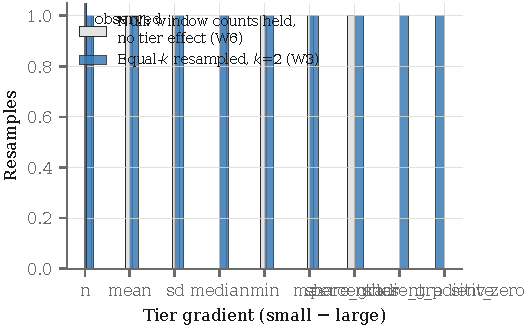
\includegraphics[width=\columnwidth]{figures/fig4_window_robustness.pdf}
  \caption{The observed gradient against two reference distributions: equal-$k$
  resampling, which removes the window-count difference, and a null in which real
  window counts are held fixed but all tier signal is destroyed.}
  \label{fig:robustness}
\end{figure}

Window count scales with filing length and so with tier ($\rho = 0.372$,
$p = 0.004$), so a filing mean averages far more windows for a large firm than a
small one. Averaging more draws reduces the variance of a mean without shifting
its expectation, but composition and window-size effects can bias it, so we tested
this directly rather than argue about it.

Equalising window counts by subsampling $k = 2$ windows per filing, the primary
sign holds in \WThreeShare{} of draws against a pre-declared threshold of 0.90:
the criterion is not met. The window-level mixed model agrees, with a
Small-vs-Large coefficient of \WFiveSmallCoef{}
[\WFiveSmallCIlo, \WFiveSmallCIhi] ($p = \WFiveSmallP$).

The sharpest result is the null simulation. Holding each filing's real window
count fixed and destroying all tier signal, unequal window counts alone produce a
Small-minus-Large gradient of 0.0218 at the 95th percentile --- \emph{larger than
the \PrimaryGradient{} we observed}, which sits at the \WSixPercentile th
percentile of that null ($p = \WSixP$). A gradient of this size is within what the
aggregation manufactures on its own.

\section{What This Means}

Under the pre-registered definition the result is a null on three independent
grounds: the confirmatory test is not significant, the tier means are not
monotone, and the window-count gate fails. We report it as the headline.

The useful reading is not that smaller firms write no more ambiguously. It is that
a filing-level measure built this way cannot answer the question. The construct
shows signal where it is computed, loses it on aggregation, and the aggregation
itself can produce a gradient of the size reported. Any study aggregating
LLM judgments over document chunks faces the same arithmetic, and we would argue
for reporting split-half reliability, an intraclass correlation, and an equal-$k$
subsampling check as a matter of routine.

\section{Limitations}

\NFirms{} firms is a measure-validation sample. Size tier stands in for a
point-in-time size measure not yet available. One model family produces the main
results. We report no market outcome. The persona prompts are a design choice, and
a different set of lenses would give a different measure. The noise-floor subset
was cut short by rate limiting and is large-cap only. Deviations from the
pre-registered plan are logged in the repository and summarised in the appendix.

\section{Conclusion}

Truncating filings to a fixed budget makes coverage a function of firm size, and
at scale nearly every 10-K is truncated under budgets in routine use. A
window-level protocol removes that confound. Applying it, our measure of
interpretive complexity is real at the window level, discriminant, and
encoder-robust --- and still too unreliable at the filing level to support the
cross-sectional claim it was built for. We report that, and the diagnostics that
establish it, as the more useful result.

\bibliographystyle{ACM-Reference-Format}
\bibliography{refs}

\end{document}
